\chapter{I/O Logic Cores and Data Synchronisation}
\label{IO_Chapter}

This chapter describes the logic cores used to communicate with the PCI Local
Bus, the video DAC, the DVI TMDS encoder, the USB UART, and the LEDs. Also
contained is the clocking and data synchronising issues that had to be solved so
that the previously mentioned logic cores can exchange data using the OpenVGA
Wishbone bus.


\section{Clock Architecture}
\label{CLOCK}
All OpenVGA clock signals are derived from either the 33~MHz PCI clock, or the
50~MHz on-board crystal oscillator (see Figure~\ref{OPENVGA_OpenVGA}). The
display dot-clock, while derived from the 50~MHz oscillator, has to be treated as a
separate clock domain since its frequency can be set to either 25~MHz or 40~MHz,
depending on the video mode.


\subsection{Spartan-3 Clocking Resources}

The Spartan-3 contains low-skew clock lines which can be connected to all the
logic resources within the FPGA. To drive these lines there are a couple of logic
primitives, \texttt{BUFGMUX} and \texttt{DCM}, that can be used.


\subsubsection{Global Clocks}

\mmodule{Patrick Suggate}{BUFGMUX, BUFG}
{Simulation modules which emulate the functionality of the Xilinx Spartan-3
primitives with the same name.} {/sim/xilinx/BUFGMUX.v, /sim/xilinx/BUFG.v}
{/sim/xilinx/BUFGMUX\_tb.v, /sim/xilinx/BUFG\_tb.v}{GPL}

The 200k-gate Xilinx Spartan-3 FPGA has eight dedicated, low-skew, global clock
lines~\cite{Xilinx_SP3_DS}. These are routed throughout the FPGA and designed
primarily for use as clock and reset signals. Skew on the clock or reset signals
can cause metastability so it is essential that skew on these lines is low, or at
least known. XST automatically calculates the skew of a synthesised design, and
generates a timing report for the clock signals. These reports also include
warnings when a design uses clock signals in a way that may cause unpredictable
skew.

Clock signals can be explicitly routed into global clock lines using the Xilinx
\texttt{BUFGMUX} primitive, though this is normally performed automatically by
XST. A \texttt{BUFGMUX} is a two input multiplexer and the output is a global
clock line. This primitive allows one of two different clock signal inputs to be
selected as the source. This primitive contains logic to avoid clock glitches so
the input source clock can be dynamically switched.


\subsubsection{Digital Clock Managers}
\label{CLOCK_DCM}

\mmodule{Patrick Suggate}{DCM}
{Simulation modules which emulate the functionality of the Xilinx Spartan-3
primitives with the same name.} {/sim/xilinx/DCM.v} {/sim/xilinx/DCM\_tb.v}{GPL}

The Spartan-3 family of FPGAs typically contain four DCM (Digital Clock Manager)
primitives, except for the smallest device which only has
two~\cite{Xilinx_SP3_DS}. DCMs use DLLs (Delay-Locked Loops) to condition clock
input signals, and optionally phase-shift and derive new clocks as well.
Conditioning the input clock signals ensures a clean clock output, corrects the
duty-cycle (optional), and allows XST to more accurately assess and control
clock-skew. Additionally, the input clock period can be multiplied and divided to
generate new clocks, and this feature was used to generate processor, SDRAM, and
VGA clocks from the on-board 50~MHz oscillator.

\begin{figure}[h!]
\begin{center}
\includegraphics[width=0.65\linewidth]{diagrams/bufgmux.pdf}
\caption[OpenVGA pixel clock generation]{BUFGMUX and DCM example showing the
OpenVGA pixel clock generation.}
\label{CLOCK_BUFGMUX}
\end{center}
\end{figure}

%  using a BUFGMUX. The pixel clock can be selected as one of two DCM outputs. The DCM has
% an optional divide-by-two parameter to halve the input clock if needed, so the
% CLK0 output is 25 MHz, and the CLKFX signal is set to output 40 MHz for use with
% the 800x600 resolution video mode

\subsection{Clock Domains}

The operating frequency of the PCI Local Bus is nominally~33 MHz~\cite{PCI_Book},
but this is not certain. There are PCI power saving modes in which the bus
frequency can be lowered, possibly even to zero\footnote{In addition,
off-the-shelf motherboard's PCI system clock can differ significantly from the
specification as the PCI clock is often derived from the Front Side Bus (FSB)
clock, which can be adjusted by the user, or differ due to manufacturing
tolerances.\cite{PCI_Book}}, for example. The video DAC and TMDS encoder ICs
operate at the dot-clock frequency, 25~MHz for the 640x480 resolution VGA. Since
these clocks differ, and also differ from the 50~MHz Wishbone bus clock, data
crossing these separate domains need to be synchronised.

The Spartan-3 FPGA has clocking resources which support clock generation and
conditioning, and multiple clock signals~\cite{SP3_DCM}. The is also logic
primitives suitable for constructing asynchronous FIFOs, a logic core used to
transfer data between clock domains.


\begin{table}[h!]
\begin{center}
\begin{tabular}{l | c c r c | c}
Clock Name & \multicolumn{4}{c|}{Clock Frequency} & Domain	\\
& \multicolumn{4}{c|}{(MHz)} & Name	\\
\hline
Wishbone Clock			& & & 50	& & Wishbone \\
CPU Clock (RISC16)		& & & 100	& & \\
CPU Clock (TTA16)		& & & 150	& & \\
SDRAM Controller Clock	& & & 50	& & \\
SDRAM Datapath Clock	& & & 100	& & \\
\hline
Video Clock 0 (640x480)	& & & 25	& & Dot Clock\\
Video Clock 1 (800x600)	& & & 40	& & \\
\hline
PCI Local Bus Clock		& & & 33	& & PCI \\
\end{tabular}
\end{center}
\label{CLOCK_Frequencies}
\caption[OpenVGA clock frequencies]{OpenVGA's clock domains and
frequencies.}
\end{table}

OpenVGA has multiple, asynchronous clock domains (see
Section~\ref{CLOCK_Async_Domains}, and data needs to be transferred between clock
domains. To prevent problems due to metastability\footnote{A full discussion of
metastability is beyond the scope of this work but a D flip-flop can enter a
metastable state if setup and/or hold times are violated. Its data output can
become essentially random.}, data crossing asynchronous clock domains needs to be
synchronised. A single-bit synchroniser is shown in Figure~\ref{CLOCK_Synchro},
and for signals many bits wide, asynchronous FIFOs (see
Section~\ref{CLOCK_Async_FIFO}) are used for synchronisation.


\subsubsection{Synchronous Clock Domains}
\label{CLOCK_Sync}

\mmodule{Patrick Suggate}{wb\_sync}
{Synchronises Wishbone transactions between two Wishbone buses with synchronous,
but different frequency, clocks.} {/rtl/lib/wb\_sync.v}
{/sim/lib/wb\_sync\_tb.v}{GPL}

Data is transported between separate OpenVGA functional units, internal to the
Spartan-3, via a Wishbone compatible bus (see Appendix~\ref{APP_Wishbone}). The
Wishbone bus clock is 50 MHz and is the DCM conditioned output generated by the
50 MHz on-board oscillator.

The CPU, SDRAM datapath, and the pixel clock, all share a common
root clock, the 50 MHz Wishbone bus clock. Though different frequencies are
used for each, the CPU (see Chapter~\ref{CPU}) and SDRAM controller (see
Section~\ref{MEM_SDRAM}) clocks are synchronous with the Wishbone bus clock,
and with frequencies that are integer multiples of the Wishbone bus clock
frequency (see Table~\ref{CLOCK_Frequencies}).

\begin{figure}[h!]
\begin{center}
\fbox{
\begin{minipage}{0.9\linewidth}
\begin{center}

\begin{tabular}{c c}
\multicolumn{2}{c}{Synchronisers for single-bit signals crossing between
different clock domains}\\
\\
Synchronous & Asynchronous	\\
\includegraphics[width=0.33\linewidth]{diagrams/synchroniser.pdf}	&
\includegraphics[width=0.44\linewidth]{diagrams/sync2.pdf}
\end{tabular}
\end{center}
\end{minipage}
}
\end{center}

\caption[Single-bit synchronisers]{A synchronisers for crossing clock domains.}
\label{CLOCK_Synchro}
\end{figure}

Transitions between these synchronous clock domains requires two DFFs (see
Figure~\ref{CLOCK_Synchro}) for each signal that crosses a domain boundary.
Additionally, signals multiple bits wide retain the same relative phase when
crossing synchronous domains using simple synchronisers, which is not the case
for crossing asynchronous domains using simple synchronisers\cite{Async_FIFO}.


There are three additional problems when crossing synchronous clock domains:
\begin{enumerate}
\item A signal crossing from the higher-frequency domain, to the slower domain, needs
to be asserted for at least one cycle of the slower clock so it is registered
correctly.
\item  When a signal crosses from the slower clock domain, to the higher frequency
clock domain, the higher frequency domain needs to correctly handle that the
signal might remain asserted for more than one cycle of the faster clock, but
should only trigger once.
\item At the boundary of two synchronous signals, the setup and hold times must
be met for both D flip-flops, which means that the smallest period of the two
timing constraints has to be applied to both DFFs.
\end{enumerate}

To solve the first two of these issues, an acknowledge (ACK) signal was used
when crossing synchronous clock domains. This indicates that a signal has been
correctly registered. The signal source then de-asserts the signal at the end of
the cycle which the ACK was received. For the final problem, XST automatically
applies the correct constraint but the designer still needs to be aware that
the tightest of the two constraints will apply to any combinatorial logic.


\subsubsection{Asynchronous Clock Domains}
\label{CLOCK_Async_Domains}
To cross asynchronous clock domains there are two common methods: a simple two
flip-flop synchroniser (see Figure~\ref{CLOCK_Synchro}), which is useful for
single bit flags like an interrupt signal; and asynchronous FIFOs, which are
useful for multiple bit-width signals, like buses, where a phase relationship
has to be maintained for all signals, across the entire width~\cite{Async_FIFO}.

\subsection{Asynchronous FIFOs}
\label{CLOCK_Async_FIFO}

\mmodule{Patrick Suggate}{afifo16, afifo2k}
{Parameterisable, asynchronous FIFOs, with either 16 or 2048 entries, which
synchronise and queue data which has to cross asynchronous clock domains.}
{/rtl/lib/fifo/afifo16.v, /rtl/lib/fifo/afifo2k.v, /rtl/lib/counter/bin2gray.v}
{/sim/lib/wb\_sync\_tb.v}{GPL}

% \begin{tabular}{l l}
% \textbf{Modules:}		& afifo16, afifo2k	\\
% \textbf{Related Files:}	& /rtl/lib/fifo/afifo16.v, /rtl/lib/fifo/afifo16.v, 	\\
% 						& /rtl/lib/counter/bin2gray.v	\\
% \textbf{Testing Files:}	& /sim/lib/fifo/afifo\_tb.v	\\
% \end{tabular}

An asynchronous FIFO takes write data from one clock domain and stores it
internally within a queue, implemented using SRAM, and the data can then be read
out to the other clock domain. The FIFO generates control signals to indicate its
state (empty, full, etc.) so that data is not written to a full FIFO, or
requested from an empty FIFO. To avoid metastability, even these control signals
are valid in just one domain. Typically the empty signal is valid in the FIFO's
read clock domain, and the FIFO's full signal is typically valid within the
FIFO's write clock domain.

The penalty due to having to use an asynchronous FIFO is both a latency penalty
and extra logic usage (approximately 60 Spartan-3 logic slices per 32-bit wide
FIFO, see Section~\ref{CLOCK_FIFO_Synth}). Asynchronous FIFOs are only used for
the PCI and the video redraw circuits since each are within separate asynchronous
clock domains.

There are two logical divisions of the design for an asynchronous FIFO: the logic
for adding data to the FIFO, and removing data from the FIFO; and the logic for
comparing the read and write pointer values across clock domains to allow the
setting of FIFO state flags.

\begin{figure}[h!]
\begin{center}
\includegraphics[width=\linewidth]{diagrams/afifo.pdf}
\caption[Simplified Asynchronous FIFO Schematic]{Simplified schematic showing
the basic components of an asynchronous FIFO.}
\label{FIFO_Logic}
\end{center}
\end{figure}

The logic for adding (and removing) data is straightforward, simply increment the
write pointer every time data is added, and increment the read pointer whenever
data is removed. Figure~\ref{FIFO_Logic} is a simplified diagram of a FIFO, the
Gray-encoders are not shown, and neither is a faster \texttt{full} and
\texttt{empty} assertion path. These are covered in detail in~\cite{Async_FIFO2}.

Comparing these pointers across clock domains, as is needed to set the
full and empty flags, is more difficult due to the possibility of
metastability. Standard base-2, ripple-carry incrementers can have multiple,
even all, bits change during an increment operation. This could potentially
cause every bit to become non-deterministic within the post-synchronised,
pointer representation.

The first step for the control signal generation is to convert the pointers into
a unit-distance representation\footnote{A unit distance encoding means that only one
bit changes between successive values in a sequence, but arithmetic in this
encoding is more complex which is why a standard representation is used for the
pointers.}, like Gray encoding, and this was used here (see
Table~\ref{CLOCK_Gray_Codes}. Even with metastability the desired pointer value
has a maximum difference of one from any generated post-synchronised pointer.
The only two values that the post-synchronised pointer can have is the previous
value or the desired value, and this will become the correct value the
following clock cycle anyway~\cite{Async_FIFO, Async_FIFO2}.

\begin{table}
\begin{center}
\begin{tabular}{| r || r | r |}
\hline
Decimal & Binary & Gray Code \\
\hline
0 & 0000 & 0000 \\
1 & 0001 & 0001 \\
2 & 0010 & 0011 \\
3 & 0011 & 0010 \\
4 & 0100 & 0110 \\
5 & 0101 & 0111 \\
6 & 0110 & 0101 \\
7 & 0111 & 0100 \\
8 & 1000 & 1100 \\
9 & 1001 & 1101 \\
10 & 1010 & 1111 \\
11 & 1011 & 1110 \\
12 & 1100 & 1010 \\
13 & 1101 & 1011 \\
14 & 1110 & 1001 \\
15 & 1111 & 1000 \\
\hline
\end{tabular}
\caption[Comparison of Decimal, Binary, and Gray Encoding.]{Gray codes with the
standard binary and decimal equivalents.}
\label{CLOCK_Gray_Codes}
\end{center}
\end{table}


\subsubsection{Control Signals}
Either the \texttt{full} or \texttt{empty} signals are asserted when the two
Gray-encoded counters match. Depending whether the the match was caused by the
FIFO going full, or going empty, determines which of the two flags is asserted.

The count order of the two Most Significant Bits\glossary{name={MSB},
description={Most Significant Bit}} (MSBs) of a Gray code counter are identical
to the two MSBs of the standard binary encoding. By sampling the two MSBs of the
Gray codes we can determine which quadrant the value is in. Using this quadrant
detection, and by comparing the current pointer values with the previous pointer
values, it can be determined whether the FIFO was going full, or going empty,
immediately before the pointers matched.


\subsubsection{Half-Full Detection}
In some applications, as with the video redraw circuit, it is useful to prefetch
multiple words, since this makes more efficient use of the Wishbone bus. Before a
prefetch is issued the prefetch control logic needs to know whether there is
space in the FIFO for the entire data transfer. An extra FIFO control signal,
calculated by comparing pointer quadrants, was added for this purpose.

By comparing the two MSBs of the FIFO read and write pointers, since these
quadrant bits have the same value as the standard binary encoding, the FIFO can
calcualte the difference in quadrants between the two pointers. If the quadrant
bits are equal then both pointers are within the same quadrant so the FIFO is
less than $25\%$, or more than $75\%$ full. If there are more than two quadrants
between the write and the read pointer, then the FIFO can also more than three
quarters full. The result is a control signal that detects whether the FIFO is
between $25\%$ and $75\%$ full (or not), and has been labelled \texttt{halfish}.


\subsubsection{Performance and Size}
\label{CLOCK_FIFO_Synth}

The size of a synthesised asynchronous FIFO, with a data width of 32-bits, and
with the target a Xilinx Spartan-3 FPGA was 59 slices\footnote{The 200k gate
Spartan-3 device that was used for OpenVGA contains 1920 logic slices}. With high
optimisation settings, the maximum speed at which the FIFO clocks is 144~MHz,
with the data write clock domain being the slowest (clock period of 6.9~ns). The
read clock domain achieved a clock period 3.8~ns, but since the logic for both
domains is very similar, this difference was speculated to be due to how XST
optimised the design.


\section{PCI-to-Wishbone Bridge}
\label{PCI}

\mmodule{Patrick Suggate}{pci\_mem\_top}
{A \textit{Plug and Play} compliant PCI-to-Wishbone-bridge logic core.}
{/rtl/pci/pci\_mem\_top.v, /rtl/pci/pci\_mem.v, /rtl/pci/cfgspace.v}
{/rtl/pci/pci\_mem\_top\_tb.v}{GPL}

OpenVGA connects to the host computer using the Peripheral Component Interconnect
(PCI) Local Bus. All data exchanged between OpenVGA and the host is through the
PCI-to-Wishbone bridge logic core. PCI was developed by Intel in 1991 as a
replacement for the aging Industry Standard Architecture (ISA)
Bus~\cite{PCI_Book, PCI_Spec}. PCI features data widths of 32 or 64 bits and has
nominal operating frequencies of 33 or 66 MHz (but can be reduced by power saving
modes).

\begin{figure}[h!]
\begin{center}
\includegraphics[width=\linewidth]{images/pci_bridge.pdf}
\end{center}
\caption[PCI-to-Wishbone bridge block diagram]{PCI-to-Wishbone bridge block
diagram.}
\label{PCI_Block_Diagram}
\end{figure}


\subsection{PCI-to-Wishbone Bridge Logic Core}
This logic core maps OpenVGA's local memory into the host-system's address space,
and this bridge allows data to pass between the host and OpenVGA.
Figure~\ref{PCI_Block_Diagram} represents a simplified diagram of this logic
core. The OpenVGA PCI bus interface is in a separate clock domain to the system
Wishbone bus. PCI typically operates at 33 MHz, with the clock signal provided by
the host system, and the Wishbone bus domain operates at 50 MHz. This clock is
generated using an on-board crystal oscillator.

The PCI bridge logic core consists of two state machines, two asynchronous FIFOs,
and some additional control and pipelining logic. Asynchronous FIFOs were used so
that data can be transferred from one clock domain to another (see
Figure~\ref{PCI_Block_Diagram}). When synchronising signals across clock domains,
these FIFOs typically add a latency penalty of two clock cycles. Domain crossing
therefore adds two cycles of latency for a PCI write and four cycles of latency
for a PCI read request.


\subsubsection{PCI-Domain State Machine}
This state machine queues PCI read and write requests, and write data, in the
PCI-to-Wishbone asynchronous FIFO. PCI read transactions require that data be
fetched from the Wishbone bus domain and placed in the Wishbone-to-PCI FIFO. The
contents of this FIFO can then be read from the PCI domain, with the data being
placed on the PCI bus. The states of this state-machine, and the signals that
cause transitions between these states, are shown in Figure~\ref{PCI_SMs}.

To prevent the PCI bridge from being overwhelmed by many back-to-back PCI write
transactions, the bridge will generate \texttt{TARGET ABORT} responses when the
bridge is already busy. Multiple PCI read requests cause no problems though. This
is because they must wait for data retrieved from the Wishbone domain before
the transaction is completed.

\begin{figure}[h!]
\begin{center}
\includegraphics[width=\linewidth]{images/pci_state_machines.pdf}
\end{center}
\caption[The PCI bridge state machines]{The PCI bridge state machines.}
\label{PCI_SMs}
\end{figure}

% The \texttt{wb{\_}busy} signal indicates there are pending writes, stored in the
% FIFO, so a PCI \texttt{TARGET ABORT} command is issued to terminate the current
% transaction, to be retried later. While in the \texttt{IDLE} state, if a PCI
% transaction is intiated by a PCI master, the address is stored in the
% PCI-to-Wishbone FIFO. \\
% In the \texttt{READ} state, any 32-bit words in the Wishbone-to-PCI FIFO are
% transferred to the PCI bus, and asserting the \texttt{TARGET READY} signal to
% indicate valid data. \\
% In the \texttt{WRITE} state, data is retreived from the PCI bus and stored in the
% PCI to Wishbone FIFO, as space allows. For every 32-bit word transfered to the
% FIFO \texttt{TARGET READY} is asserted.


% \begin{figure}[h!]
% \begin{center}
% \includegraphics[width=\linewidth]{diagrams/pci_pci_state_machine.eps}
% \end{center}
% \caption[PCI clock domain state machine]{PCI clock domain state machine.}
% \label{PCI_PCI_SM}
% \end{figure}


\subsubsection{Wishbone-Domain State Machine}
The PCI-to-Wishbone FIFO's \texttt{empty} signal de-asserting indicates that
there is a PCI request pending. The Wishbone-side state machine decodes this
request and issues a corresponding Wishbone transaction. Reads result in data
being transferred to the PCI domain using the Wishbone-to-PCI asynchronous FIFO,
writes use the PCI-to-Wishbone FIFO to transfer data to the Wishbone domain.

Summary of this state's machines signals:
\begin{itemize}
  \item \texttt{empty}: Indicates the PCI-to-Wishbone FIFO is empty. When this
  signal de-asserts, there are pending PCI transactions to process, causing the
  state-machine to transition to the \texttt{ADDR} state. When this signal
  asserts in the \texttt{WRITE} state all data have been transferred, ending
  the write transaction.
  \item \texttt{cmd\_rd}: When in the \texttt{ADDR} state, this signal causes a
  transition to the \texttt{READ} state, causing a Wishbone read transaction to
  be issued.
  \item \texttt{cmd\_wr}: When in the \texttt{ADDR} state, this signal causes a
  transition to the \texttt{WRITE} state, causing a Wishbone write transaction
  to be issued.
  \item \texttt{wb\_end}: Indicates the end of a Wishbone transaction,
  triggering a return to the \texttt{IDLE} state when in the \texttt{READ}
  state.
\end{itemize}
% When the PCI-to-Wishbone asynchronous FIFO is not empty there are pending PCI
% requests (see Figure~\ref{PCI_WB_SM}). The first step is to read the command and
% address out of the FIFO, and fetch data if the command is a  read, placing read
% data it into the Read Data FIFO (RDF), or keep reading data from the
% PCI-to-Wishbone FIFO, and sending the data out over the Wishbone bus.

% Within the Wishbone clock domain, for the PCI module. The first item to be read
% from the PCI to Wishbone FIFO contains the command and the address information.
% The state machine transitions to the \texttt{ADDR} state to latch the address and
% determine the next state, either \texttt{WRITE} or
% \texttt{READ}. \\
% The \texttt{WRITE} state transfers data from the PCI bus to the
% Wishbone bus. PCI burst transfers are supported but all Wishbone operation are atomic. \\
% The \texttt{READ} state fetches a single 32-bit word from main memory, via the
% Wishbone bus, placing it upon the PCI bus, then returning to the \texttt{IDLE}
% state upon completion.

% \begin{figure}[h!]
% \begin{center}
% \includegraphics[width=\linewidth]{diagrams/pci_wb_state_machine.eps}
% \end{center}
% \caption[Wishbone clock domain state machine for the PCI module]{The
% Wishbone clock domain state machine of the PCI bridge.}
% \label{PCI_WB_SM}
% \end{figure}


\subsubsection{PCI Configuration Space}
Upon system start-up, each PCI function and device has its configuration space
registers read to determine its capabilities. The host (BIOS or operating system)
can choose to write to configuration space registers to map the PCI device's
registers and memories into the system's memory or I/O address
spaces\footnote{I/O space is a legacy feature from early IBM-compatible x86
architectures. The PCI specification encourages the use of memory address space
instead\cite{PCI_Spec, PCI_Book}}. Figure~\ref{PCI_CFG_Cap} shows a configuration
space \texttt{WRITE} access generated by a \textit{Plug and Play} BIOS.

It is this configuration space information that informs a \textit{Plug and Play}
BIOS as to whether a device is a VGA-compatible video controller, a network
interface card, or any other category of device listed in~\cite{PCI_Spec}. To be
VGA-compatible, OpenVGA can be synthesised with VGA configuration space settings.


\subsection{PCI Testing and Summary}
The PCI specifications expect a device to respond within 25 clock
cycles~\cite{PCI_Spec}, and since four PCI cycles will be consumed for data to
cross clock domains and resynchronise, this means that the OpenVGA has only 630
ns to complete the request and signal \texttt{TARGET READY}\footnote{There is a
PCI command \texttt{TARGET ABORT} which is effectively ``try again later''. This
command is issued whenever there is still write data within the PCI to Wishbone
asynchronous FIFO. The rest of the time all PCI accesses are routed to the SDRAM
controller via the Wishbone bus and are expected to complete within this 630
ns.}.

\begin{figure}[h!]
\begin{center}
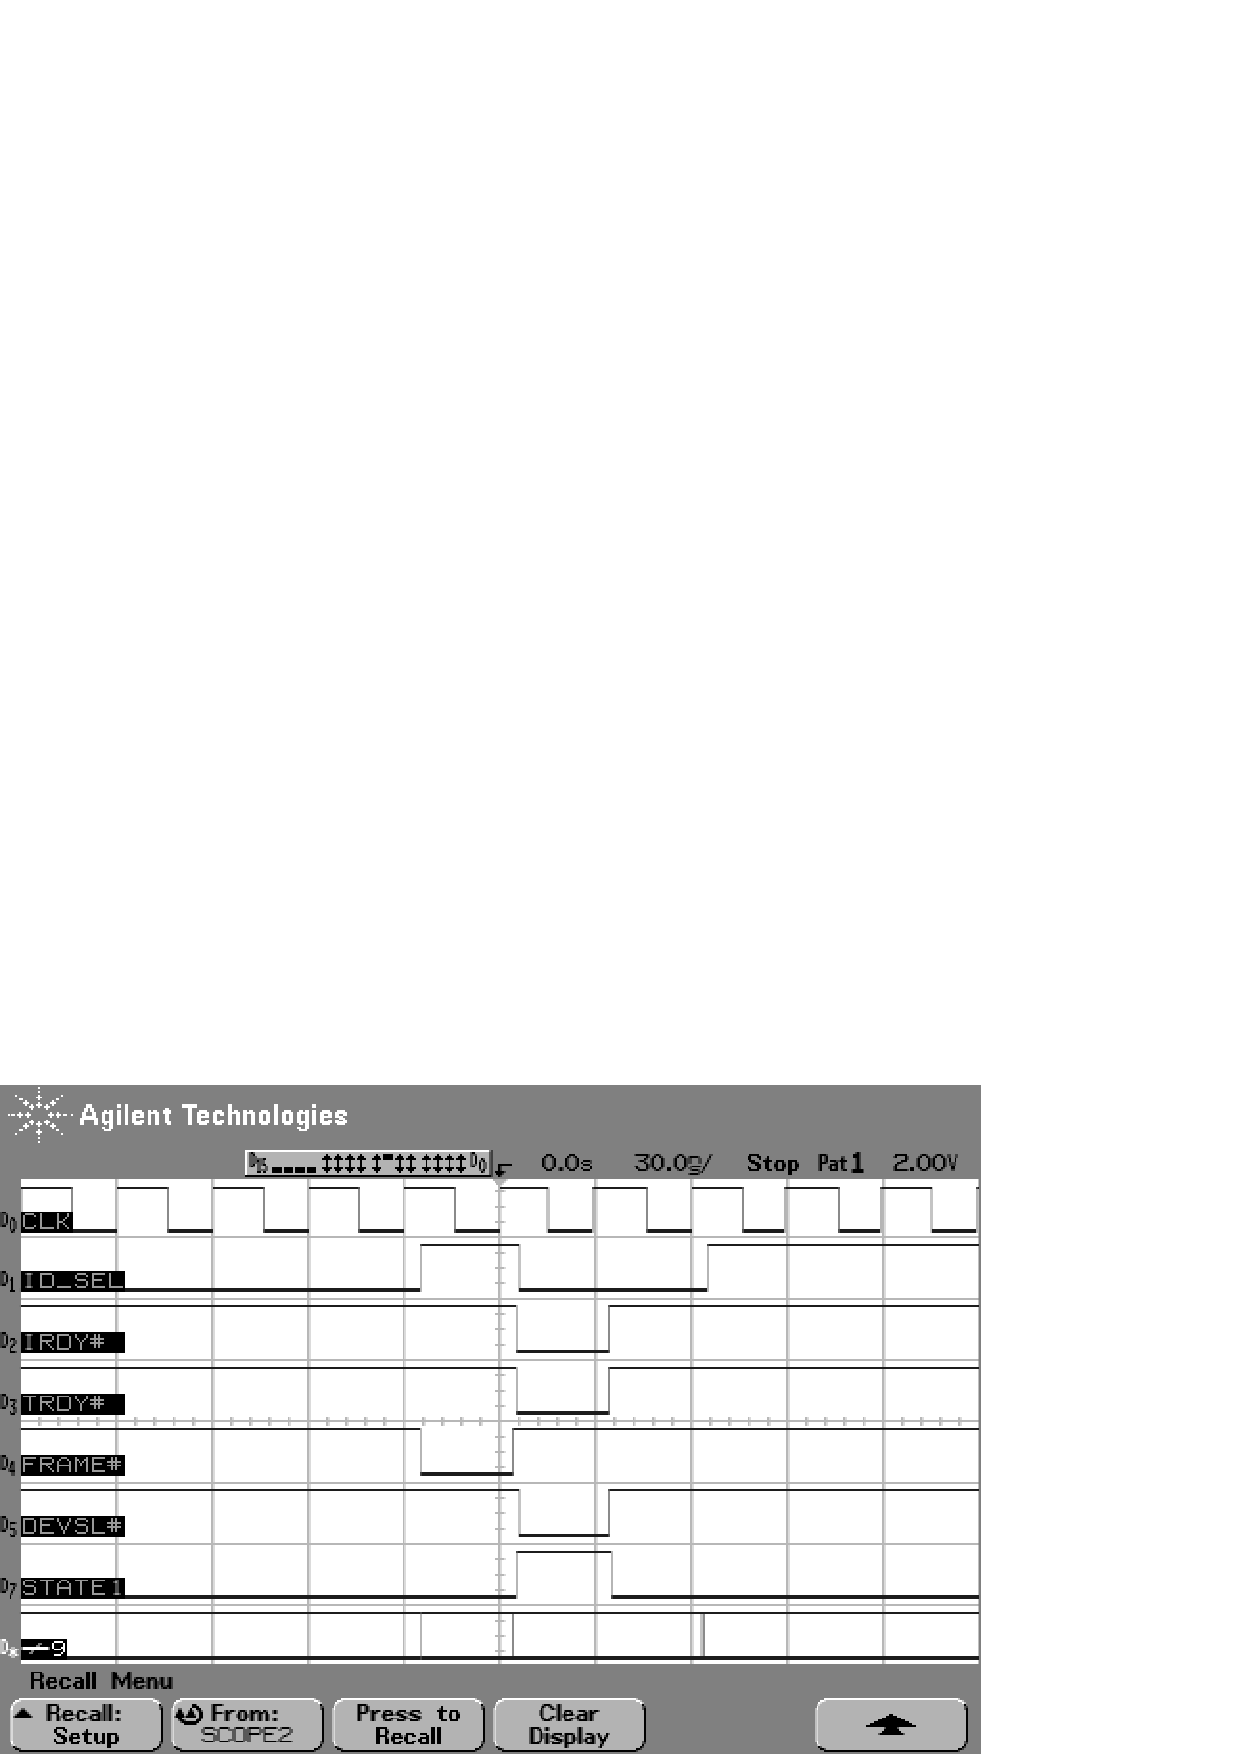
\includegraphics[width=\linewidth]{images/cfg_space_cap.pdf}
\end{center}
\caption[PCI configuration space write transaction]{Screen capture of a PCI
configuration space write transaction.}
\label{PCI_CFG_Cap}
\end{figure}


\section{VGA and DVI Controller}
\label{VIDEO}

\mmodule{Patrick Suggate}{wb\_video\_top}
{This logic core reads 16-bit pixel data from the framebuffer and converts it to
24-bit colour, outputing this to the video DAC and TMDS encoder, as well as
generating all of the other signals necessary for redrawing the display.}
{/rtl/video/wb\_video\_top.v, /rtl/video/wb\_vga\_ctrl.v,
/rtl/video/wb\_redraw.v, /rtl/video/wb\_crtc.v, /rtl/video/crtc.v,
/rtl/video/vga16.v, /rtl/lib/fifo/afifo2k.v, /rtl/video/dvi\_ctrl.v}
{/sim/video/vga\_tb.v, /sim/video/crtc\_tb.v, /sim/xilinx/DCM.v,
/sim/xilinx/BUFGMUX.v}{GPL}

OpenVGA outputs image data, made up of multiple picture elements (called
``pixels''), to a standard computer display, typically a VGA connected CRT
monitor or a VGA or DVI connected LCD monitor. The VGA standard is analogue, so a
video DAC is used, the Philips TDA8777 IC -- since the Spartan-3 has no analogue
output pins, and DVI is a serial digital interface -- encoded using a TMDS
transmitter IC, via the Texas Instruments TFP410.

VGA and DVI display formats are 2D (2-Dimensional) and multicolour, and both the
VGA and DVI use similar control and synchronisation pulses\footnote{This was
intentional to accelerate the adoption of the newer DVI
specification\cite{VESA_DVI}.}. The display data, in graphical modes, is laid out
in memory as a flattened 2D array of pixel colours. To draw a complete screen of
data, this pixel colour information is sent, one pixel at a time, to the display,
using either a VGA or DVI connection. Display update rate is typically 60~Hz,
meaning that the display is completely redrawn 60 times per second.

The block of memory that stores the pixels for a 2D display is called a
frame-buffer. The size of this memory depends on the screen resolution and the
colour depth (and can be from 1-bit to 32-bits per pixel).

\begin{figure}[h!]
\begin{center}
\includegraphics[width=\linewidth]{images/video_controller.pdf}
\end{center}
\caption[Video controller block diagram]{Video controller block diagram.}
\label{VIDEO_Ctrl}
\end{figure}


\subsection{Display Modes}

\subsubsection{Text Mode}
The original IBM VGA had hardware accelerated text modes that converted ASCII
characters, and an additional attribute byte, into pixel data as the screen was
being redrawn. This allowed a very small block of memory to represent the pixels
of an entire screen of text data. Additionally, the ASCII to pixel conversion is
quite slow on a general purpose CPU, and would have been prohibitively so in
1981~\cite{VGA_Programmers}, which is why the original IBM Monochrome Display
Adapter (MDA), and subsequent display adapters, used dedicated logic for the
task.

OpenVGA does not use legacy dedicated hardware for this ASCII to pixel conversion
as the on-board processor is capable of performing this task\footnote{The
original IBM XT ran at only 4.77 MHz, and required multiple clock cycles to
execute a single instruction, and had quite a slow system bus\cite{SVGA_Book}.
TTA16 can operate at up to 190 MHz, executes an ALU operation every clock cycle,
and has a fast connection to the framebuffer.} OpenVGA's firmware will contain
the code necessary for the ASCII to pixel transformation.
Appendix~\ref{Source_Code} contains the text-mode routines written in C. Assembly
for both RISC16 and TTA16 was written, based upon the C code, and used to
evaluate each processor.

\begin{figure}[h!]
\begin{center}
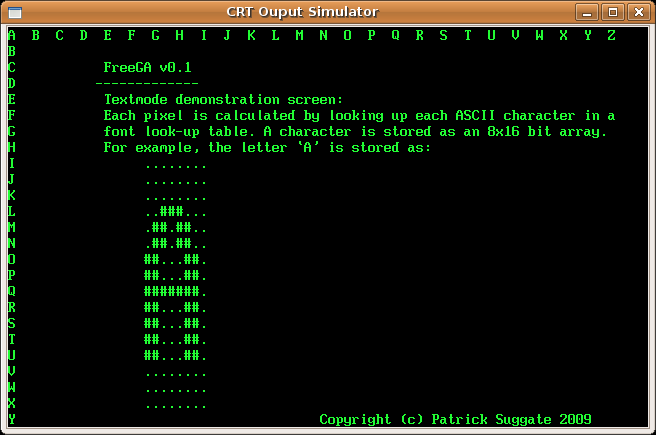
\includegraphics[width=\linewidth]{images/crt_sim.png}
\caption[Emulated text-mode display data produced by a simulation]{Emulated
text-mode display data produced by a simulation.}
\label{CRT_Sim}
\end{center}
\end{figure}

To display the output of simulations of text mode, a Python script was written
that takes in the generated pixel data and displays it in a window. The results
produced by both the Icarus Verilog test-harnesses and the C code can then be
verified. A screen capture of the generated text-mode output is shown in
Figure~\ref{CRT_Sim}.

\subsubsection{Graphic Modes}
\label{VIDEO_Modes}
The current version of OpenVGA has only two frequencies available as the clock
source for the display timing, 25 MHz and 40 MHz. Table~\ref{VIDEO_Modes_Table}
shows common modes which use these dot clock frequencies.


\begin{table}[h!]
\begin{center}
\begin{tabular}{l r r r l}
				& 640x400	& 640x480	& 800x600	& Unit	\\
				& (VGA text)& (VGA)		& (SVGA)	&		\\
\hline
\textit{General Timings}	&	&	&	& \\
Dot Clock		&	25		&	25		&	40		& MHz	\\
H-sync			&	31.5	&	31.5	&	37.9	& kHz	\\
V-sync			&	70		&	60		&	60		& Hz	\\
Redraw data rate&	36.9	&	34.6	&	57.6	& MB/s	\\
\textit{Horizontal Timings}	&	&	&	& \\
Front porch		&	16		&	16		&	40		& clock cycles	\\
Back porch		&	48		&	48		&	88		& clock cycles	\\
H-sync duration	&	96		&	96		&	128		& clock cycles	\\
H-total			&	800		&	800		&	1056	& clock cycles	\\
\textit{Vertical Timings}	&	&	&	& \\
Front porch		&	12		&	10		&	1		& clock cycles	\\
Back porch		&	35		&	33		&	23		& clock cycles	\\
V-sync period	&	2		&	2		&	4		& clock cycles	\\
V-total			&	449		&	525		&	628		& clock cycles	\\
\end{tabular}
\end{center}
\caption[OpenVGA video modes]{OpenVGA video modes which use a dot-clock of
either 25 MHz or 40 MHz.}
\label{VIDEO_Modes_Table}
\end{table}

\subsection{Pixel Data Prefetch}
\label{VID_Prefetch}

The OpenVGA display data is stored in the SDRAM, which is in the Wishbone clock
domain, and needs to be prefetched and queued within the dot-clock domain for
redrawing the display. The data needs to be prefetched since the SDRAM is shared
with other peripherals but a steady stream of data is needed to redraw the
display without artifacts\footnote{The required data rate to redraw the display,
at a resolution of 640x480, and 16-bit colour, is 50 MB/s. Pixel data has to be
ready at each edge of the dot-clock when redrawing or else that pixel is
skipped.}

A 2 kB asynchronous FIFO achieves both these requirements, synchronises data
which has to cross clock domains, and queues up a large quantity of pixel data so
redraw can occur uninterrupted. The FIFO's half-full signal is used to trigger
prefetches, which are always 256 byte burst read transfers from the SDRAM
controller, as this is the SDRAM column size with the 8 MB SDRAM that was used.


\subsubsection{Video Clocks}
The signals to drive a display device, like a monitor, exist in their own clock
domain as well. This is because different video modes typically use different
pixel clocks to fetch and display pixel data, therefore has to be decoupled from
the system's internal bus clock. For example, the display mode 640x480 @60 Hz
uses a 25.175 MHz clock, 800x600 @60 Hz uses a 40 MHz clock, and 1024x768 @60 Hz uses
a 65 MHz clock. To transfer data from the clock domain of the system's Wishbone
bus to the video redraw circuit's clock domain, another asynchronous FIFO is
needed, but only one since data is transferred in just one direction. This
asynchronous FIFO was implemented using a BRAM and also functions as a prefetch
queue (see Section~\ref{VID_Prefetch}).


\subsection{CRT Controller}
\label{VID_CRTC}

The CRT Controller (Cathode Ray Tube Controller, called this for historic
reasons) generates the horizontal and vertical refresh signals which determine
the display resolution. To redraw the display, pixels are drawn from the top
left to the bottom right of the display\cite{VGA_Programmers} (see
Figure~\ref{INTRO_CRT_Redraw}). The display is redrawn row-by-row with a
horizontal synchronisation pulse marking the end of every row. Once all rows have
been redrawn, a vertical synchronisation pulse marks the end of the screenful of
data.

The basic design of the CRTC is two counters, a column counter and a row counter.
The column counter increments at each positive edge of the dot-clock until the
column limit is reached and then restarts at zero. Every time the column counter
resets to zero, the row counter increments until it reaches its row limit, and
then resets to zero.


\subsection{VGA Output}
\label{VIDEO_VGA_Output}

OpenVGA's output to a VGA monitor are three analogue colour components (red,
green, and blue), the horizontal synchronisation signal (subsequently referred to
as hsync), and the vertical synchronisation signal (subsequently referred to as
vsync).

The analogue signals are generated by an external video DAC since the Spartan-3
has no analogue outputs. The video DAC is connected to the Spartan-3 in 24-bit
colour mode, and since OpenVGA's framebuffer is stored as 16-bit colour data, to
reduce memory bandwidth, this data has its Least Significant
Bits\glossary{name={LSB}, description={Least Significant Bit}} (LSBs) padded with
zeros.


\subsection{DVI Output}
\label{VIDEO_DVI_Output}

The DVI transmitter IC is connected to the Spartan-3 in 12-bit DDR mode, which
means half the 24-bit colour is transferred on each clock edge. DVI support is
incomplete and the DVI output functionality has been only partially simulated but
not tested on OpenVGA hardware due to time constraints.


\section{Miscellaneous Peripherals}

\subsection{LEDs}
\label{LED_Driver}

\mmodule{Patrick Suggate}{wb\_leds}
{MMIO module for driving on-board LEDs.} {/rtl/lib/wb\_leds.v}
{/sim/lib/wb\_leds\_tb.v}{GPL}

OpenVGA has two LEDs for diagnostic and debugging output. These are memory-mapped
to the address 0x480000 . The following listing is a TTA16 assembly routine from
the OpenVGA firmware that sets the LEDs.

\begin{center}
\begin{minipage}{0.8\linewidth}
\footnotesize
\verbatiminput{source/tta16_set_leds.tex}
\normalsize
\end{minipage}
\end{center}

% \begin{lstlisting}[language={[x86masm]Assembler}]
% ; set_leds - The two LSBs of `r0' determines the LED outputs.
% set_leds:	{		,		,		,1	}
% 		{		,		,com	->msr	,0x48	}
% 		{\r0	->wad	,		,\r0	->mem	,1	}
% 		{\r15	->bra	,		,com	->msr	,\r12	} ; Restore SS
% 		{		,		,		,	}
% \end{lstlisting}


\subsection{USB Serial Port}
\label{USB_Sport}

\mmodule{Jeung Joon Lee, Patrick Suggate}{wb\_serial\_port}
{A Wishbone interface to a standard UART.} {/rtl/lib/wb\_serial\_port.v,
/rtl/lib/uart/*} {/sim/lib/wb\_serial\_port\_tb.v}{Modified BSD, GPL}

A USB port was also included as part of the OpenVGA hardware. This is connected
to the FPGA via a FTDI serial port IC. The Wishbone module allows the CPU to send
and receive data via the serial port, with the goal of being able to dump
OpenVGA's state, to aid with debugging OpenVGA.

The UART modules used as part of \texttt{wb\_serial\_port} is an open source
module, with a very permissive license, and was obtained from OpenCores.org, a
repository of open source HDL modules. The baud rate is configurable in the
Verilog code and currently operates at 9600 baud, 8-bits data, one stop-bit, and
no parity-bit.
